% Harus dimuat terlebih dahulu, digunakan agar file PDF memiliki format karakter yang benar.
% Untuk informasi lebih lanjut, lihat https://ctan.org/pkg/cmap.
\RequirePackage{cmap}

% Format dokumen sebagai paper konferensi menggunakan aturan IEEEtran terbaru (v1.8b).
% Untuk informasi lebih lanjut, lihat http://www.michaelshell.org/tex/ieeetran/.
\documentclass[conference]{IEEEtran}[2015/08/26]

% Format encoding font dan input menjadi 8-bit UTF-8.
\usepackage[T1]{fontenc}
\usepackage[utf8]{inputenc}

% Format bahasa menjadi bahasa german dan inggris.
\usepackage[indonesian]{babel}

% Digunakan untuk tujuan demonstrasi.
\usepackage{mwe}

% Digunakan untuk menampilkan font dengan style yang lebih baik.
\usepackage[zerostyle=b,scaled=.75]{newtxtt}

% Digunakan untuk menampilkan tabel dengan style yang lebih baik.
\usepackage{booktabs}

% Digunakan untuk menampilkan gambar pada dokumen.
\usepackage{graphicx}

% Digunakan untuk menampilkan potongan kode.
\usepackage{listings}
\lstset{
  basicstyle=\ttfamily,
  columns=fixed,
  basewidth=.5em,
  xleftmargin=0.5cm,
  captionpos=b
}

% Digunakan agar backticks (`) dapat dirender pada PDF.
% Untuk informasi lebih lanjut, lihat https://tex.stackexchange.com/a/341057/9075.
\usepackage{upquote}

% Digunakan untuk menyeimbangkan bagian akhir dokumen dengan dua kolom.
\usepackage{balance}

% Digunakan untuk menampilkan pustaka.
\usepackage[square,comma,numbers,sort&compress]{natbib}

% Mengubah format ukuran teks pada natbib.
\renewcommand{\bibfont}{\normalfont\footnotesize}

% Menambah nama penulis ketika menggunakan perintah \citet.
% Untuk informasi lebih lanjut, lihat https://tex.stackexchange.com/a/76075/9075.
\usepackage{etoolbox}
\makeatletter
\patchcmd{\NAT@test}{\else \NAT@nm}{\else \NAT@hyper@{\NAT@nm}}{}{}
\makeatother

% Digunakan untuk menambah hyperlink pada referensi.
\usepackage{hyperref}

% Menonaktifkan warna dan bookmark pada hyperref.
\hypersetup{hidelinks,
  colorlinks=true,
  allcolors=black,
  pdfstartview=Fit,
  breaklinks=true
}

% Digunakan untuk membenarkan hyperref pada gambar.
\usepackage[all]{hypcap}

% Digunakan untuk menampilkan beberapa gambar
\usepackage[caption=false,font=footnotesize]{subfig}

\usepackage{stfloats}

% Tambahkan format tanda hubung yang benar di sini
\hyphenation{
  ro-ket
  me-ngem-bang-kan
  per-hi-tu-ngan
}

\begin{document}

  % Ubah kalimat berikut sesuai dengan judul penelitian.
\title{Deteksi Berita Palsu Otomatis Berbahasa Indonesia Menggunakan BERT}

% Ubah kalimat-kalimat berikut sesuai dengan nama, institusi, alamat dan kontak penulis.
\author{
  \IEEEauthorblockN{Reza Fuad Rachmadi}
  \IEEEauthorblockA{Departemen Teknik Komputer\\
    Fakultas Teknologi Elektro\\
    dan Informatika Cerdas\\
    Institut Teknologi Sepuluh Nopember\\
    Surabaya, Indonesia 60111\\
    fuad@te.its.ac.id}

  \and
  \IEEEauthorblockN{Mauridhi Hery Purnomo}
  \IEEEauthorblockA{Departemen Teknik Komputer\\
    Fakultas Teknologi Elektro\\
    dan Informatika Cerdas\\
    Institut Teknologi Sepuluh Nopember\\
    Surabaya, Indonesia 60111\\
    hery@ee.its.ac.id}

  \and
  \IEEEauthorblockN{Aufa  Nabil Amiri}
  \IEEEauthorblockA{Departemen Teknik Komputerr\\
    Fakultas Teknologi Elektro\\
    dan Informatika Cerdas\\
    Institut Teknologi Sepuluh Nopember\\
    Surabaya, Indonesia 60111\\
    aufa.17072@mhs.its.ac.id}
}

% Digunakan untuk menampilkan judul dan deskripsi penulis.
\maketitle

  % Mengubah keterangan `Abstract` ke bahasa indonesia.
% Hapus bagian ini untuk mengembalikan ke format awal.
\renewcommand\abstractname{Abstrak}

\begin{abstract}

  % Ubah paragraf berikut sesuai dengan abstrak dari penelitian.
  Berita palsu atau yang biasa disebut hoaks adalah suatu yang hal yang sering melanda Indonesia. Dengan adanya sosial media, suatu berita palsu dapat memiliki tingkat penyebaran yang sangat luas. Selain itu, masyarakat Indonesia memiliki tingkat kecenderungan untuk menyebarkan berita palsu yang cukup tinggi. Sehingga, suatu metode pendeteksi berita palsu harus ada. Penelitian ini memanfaatkan algoritma BERT yang digunakan untuk mendeteksi apakah suatu berita adalah berita hoaks atau tidak secara otomatis. Dari suatu teks yang mentah, akan dilakukan tokenisasi sebelum akhirnya dimasukkan ke dalam algoritma BERT. Selanjutnya, keluaran dari BERT akan dijadikan sebagai inputan dari algoritma klasifikasi Linear Regression.  Barulah pada saat ini, kita bisa mendapatkan klasifikasi apakah suatu teks itu berupa berita hoaks atau tidak. Tujuan dari penelitian ini adalah untuk membuat sebuah model yang dapat digunakan untuk melakukan klasifikasi suatu teks apakah termasuk ke dalam berita hoaks atau tidak.

\end{abstract}

% Mengubah keterangan `Index terms` ke bahasa indonesia.
% Hapus bagian ini untuk mengembalikan ke format awal.
\renewcommand\IEEEkeywordsname{Kata kunci}

\begin{IEEEkeywords}

  % Ubah kata-kata berikut sesuai dengan kata kunci dari penelitian.
  BERT, Hoaks, Klasifikasi, Linear Regression

\end{IEEEkeywords}


  % Ubah bagian berikut sesuai dengan konten-konten yang akan dimasukkan pada dokumen
  % Ubah judul dan label berikut sesuai dengan yang diinginkan.
\section{Latar Belakang}
\label{sec:latarbelakang}

% Ubah paragraf-paragraf pada bagian ini sesuai dengan yang diinginkan.

Pesatnya perkembangan roket yang merupakan \lipsum[2-4]

Pembahasan pada paper ini dimulai dengan presentasi mengenai penelitian lain (Bagian \ref{sec:penelitianterkait}).
Kemudian dilanjutkan dengan penjelasan mengenai desain dan implementasi dari sistem yang dibuat (Bagian \ref{sec:desainimplementasi}).
Berdasarkan hal tersebut, kami menunjukkan lorem ipsum (Bagian \ref{sec:loremipsum}).
Terakhir, didapatkan kesimpulan dari penelitian yang telah dilakukan (Bagian \ref{sec:kesimpulan}).

  % Ubah judul dan label berikut sesuai dengan yang diinginkan.
\section{Penelitian Terkait}
\label{sec:penelitianterkait}

Sudah terdapat beberapa penelitian yang pernah dilakukan oleh orang lain mengenai pendeteksi berita hoaks ini. Aggarway et al. pernah melakukan penelitian untuk membandingkan antara BERT, XGBoost dan LSTM untuk melakukan klasifikasi berita palsu berbahasa inggris. Dari penelitian tersebut didapatkan bahwa BERT memiliki tingkat akurasi yang lebih tinggi apabila dibandingkan dengan XGBoost dan LSTM \cite{bert_news_classi}. Bahad et al. melakukan penelitian yang membandingkan antara CNN, RNN, \textit{uni-directional} LSTM RNN dan \textit{bi-directional} LSTM RNN. Hasil dari penelitian tersebut menunjukkan bahwa penggunaan LSTM ditambah dengan \textit{attention} baik itu \textit{uni-directional} maupun \textit{bi-directional} memiliki tingkat akurasi yang lebih tinggi apabila dibandingkan dengan CNN atau RNN \cite{bahad_lstm}. Dari kedua penelitian tersebut, dapat diambil kesimpulan bahwa algoritma yang 'mengingat' atau mengetahui suatu konteks dalam teks akan memiliki tingkat akurasi yang lebih tinggi dibanding algoritma dengan pendekatan yang lain.

Untuk penelitian pendeteksi berita hoaks dengan berbahasa indonesia, terdapat beberapa penelitian yang pernah dilakukan seperti oleh Prasetijo et al. yang meneliti penggunaan SVM dan SGD untuk mendeteksi berita hoaks berbahasa indonesia. Penelitian tersebut berhasil membuat suatu model dengan tingkat akurasi sebesar 85\% \cite{prasetijo}. Penelitian lain yang dilakukan oleh Rahutomo et al. dengan menggunakan algoritma \textit{naive bayes} berhasil menghasilkan akurasi sebesar 80\% \cite{rahutomo}.

  % Ubah judul dan label berikut sesuai dengan yang diinginkan.
\section{Desain dan Implementasi Sistem}
\label{sec:desainimplementasi}

% Ubah paragraf-paragraf pada bagian ini sesuai dengan yang diinginkan.

Pada cetak biru yang tertera pada Gambar \ref{fig:cetakbiru}. \lipsum[8]

% Contoh input gambar pada kolom.
\begin{figure} [ht]
  \centering
  % Ubah sesuai dengan nama file gambar dan ukuran yang akan digunakan.
  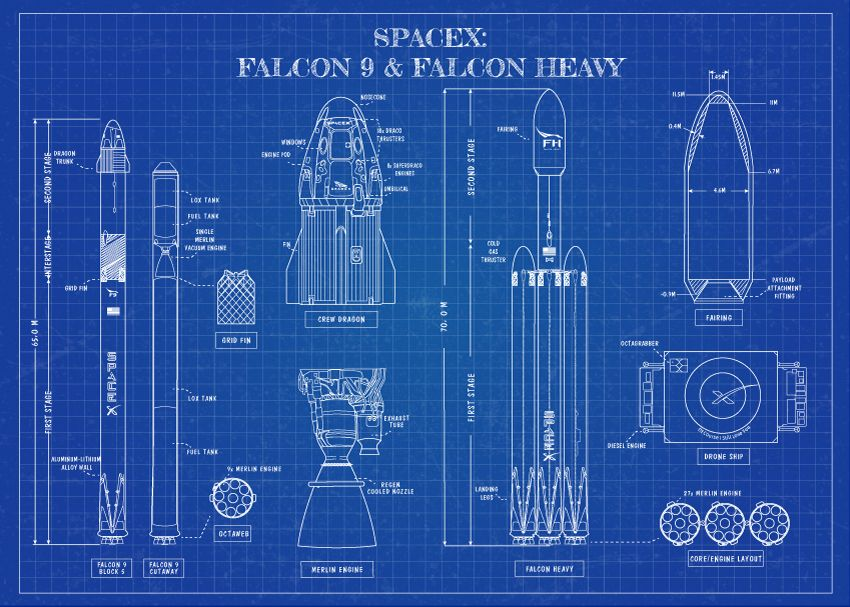
\includegraphics[width=0.4\textwidth]{gambar/cetakbiru.jpg}

  % Ubah sesuai dengan keterangan gambar yang diinginkan.
  \caption{Cetak biru roket yang akan diuji coba. \cite{cetakbiruspacex}}
  \label{fig:cetakbiru}
\end{figure}

\lipsum[9-11]

% Contoh pembuatan tabel.
\begin{table}
  \caption{Contoh tabel sederhana}
  \label{tab:tabelsederhana}
  \centering
  \begin{tabular}{lll}
    \toprule
    Heading1 & Heading2 & Heading3  \\
    \midrule
    One      & Two      & Three     \\
    Four     & Five     & Six       \\
    \bottomrule
  \end{tabular}
\end{table}

% Contoh pembuatan potongan kode.
\begin{lstlisting}[
  language=C++,
  caption={Program halo dunia.},
  label={lst:halodunia}
]
#include <iostream>

int main() {
    std::cout << "Halo Dunia!";
    return 0;
}
\end{lstlisting}

\lipsum[12]

% Contoh pembuatan daftar.
\begin{enumerate}
  \item \lipsum[13][1-4]
  \item \lipsum[13][5-8]
  \item \lipsum[13][9-12]
\end{enumerate}

\lipsum[14-15]

  % Ubah judul dan label berikut sesuai dengan yang diinginkan.
\section{Lorem ipsum}
\label{sec:loremipsum}

% Ubah paragraf-paragraf pada bagian ini sesuai dengan yang diinginkan.

% Contoh input beberapa gambar pada halaman.
\begin{figure*}
  \centering
  \subfloat[Hasil A]{\includegraphics[width=.4\textwidth]{example-image-a}
    \label{fig:hasila}}
  \hfil
  \subfloat[Hasil B]{\includegraphics[width=.4\textwidth]{example-image-b}
    \label{fig:hasilb}}
  \caption{Contoh input beberapa gambar.}
  \label{fig:hasil}
\end{figure*}

\lipsum[16-18]

% Contoh input potongan kode dari file.
\lstinputlisting[
  language=Python,
  caption={Program perhitungan bilangan prima.},
  label={lst:bilanganprima}
]{program/bilangan-prima.py}

\lipsum[19-20]

  % Ubah judul dan label berikut sesuai dengan yang diinginkan.
\section{Kesimpulan}
\label{sec:kesimpulan}

% Ubah paragraf-paragraf pada bagian ini sesuai dengan yang diinginkan.

\lipsum[21-23]


  % Menampilkan daftar pustaka dengan format IEEE
  \bibliographystyle{IEEEtranN}
  \bibliography{pustaka/pustaka.bib}

  % Menyeimbangkan bagian akhir di kedua kolom
  \balance

\end{document}
